% This is samplepaper.tex, a sample chapter demonstrating the
% LLNCS macro package for Springer Computer Science proceedings;
% Version 2.20 of 2017/10/04
%
\documentclass[runningheads]{llncs}
%
\usepackage{graphicx}
% Used for displaying a sample figure. If possible, figure files should
% be included in EPS format.
%
% If you use the hyperref package, please uncomment the following line
% to display URLs in blue roman font according to Springer's eBook style:
% \renewcommand\UrlFont{\color{blue}\rmfamily}

\begin{document}
%
\title{ARQUS Cybersecurity Summer School 2021}
%
%\titlerunning{Abbreviated paper title}
% If the paper title is too long for the running head, you can set
% an abbreviated paper title here
%
\author{Kushagra Singh BISEN\inst{1,2}}
%
\authorrunning{Kushagra Singh BISEN}
% First names are abbreviated in the running head.
% If there are more than two authors, 'et al.' is used.
%
\institute{Universit\'e Jean Monnet, Saint Etienne \and
MINES Saint Etienne, Saint Etienne \\
\email{kushagra.bisen@etu.univ-st-etienne.fr}}
%
\maketitle              % typeset the header of the contribution
%
\begin{abstract}
The document presents the solutions to the challenges given during the ARQUS Cybersecurity summer school held
from 6th to 10th September 2021. The event was hosted by universities located in Italy, France, Lithuania and Spain.
The event promoted collaboration between universities and promoted research across Europe. 4 different sections are detailing each section, concluding with the skills learnt by myself during 4 days.
\keywords{ARQUS  \and Cybersecurity \and Summer-School}
\end{abstract}

\section{Introduction}
Cybersecurity is an important growing field with the increasing number of electronic devices. As such devices are in constant interaction with humans exchanging data, security is a foremost requirement. Cybersecurity deals with preventing attacks as well as finding solutions to
encrypted problems. In the sections, we discuss the different challenges and solutions to those.

\section{Security in Android Applications}
\subsection{Introduction}
Android smartphones are the most popular versions of the modern smartphone. There are around 3 billion android smartphones active across the world. By using popular software, the risk of being exploited by unwanted users is tremendously huge. Malware can be used to control/exploit millions of users even if the malware's
reach was not big. Cybersecurity experts, responsible for the security of users plan to tackle the issue in two different ways,
1) Ensuring illegal code practices are not followed. 2) Using analysis tools to check if the application being used is safe. During the first day of our security in android application challenge, we were advised to use two different tools to analyze the coding practices as well as the security of the application being used. Subsequent sections will describe the tools being used and present results from the analysis of the tools.

\subsubsection{What is Android?}
Android can be considered an extension to the existing Java JVM library with tools to develop applications.
Android follows a layered architecture \ref{fig1} with an application layer containing the applications for the users.
A user never goes further than the application layer, whereas the developers can exploit the other layers based upon the requirement.
Since Android 6.0, Android provides the option for the user to decide if a particular application has the \textbf{permission} 
to use specific resources in the device. Malicious applications try to extract information by using permissions they do not need but use for data mining applications. Android assigns a specific Linux User ID to every application on installation. There are 130 different types of permissions an application can ask from the user. They are divided into categories, namely, 1) \textit{Normal}, basic permissions which are automatically granted
by Android. 2) \textit{Dangerous}, permissions required to access important core APIs of Android. 3) \textit{Signature}, permissions which are granted by the developer of the application itself.
4) \textit{SignatureOrSystem}, permissions which granted to the system apps automatically. 
\begin{figure}
    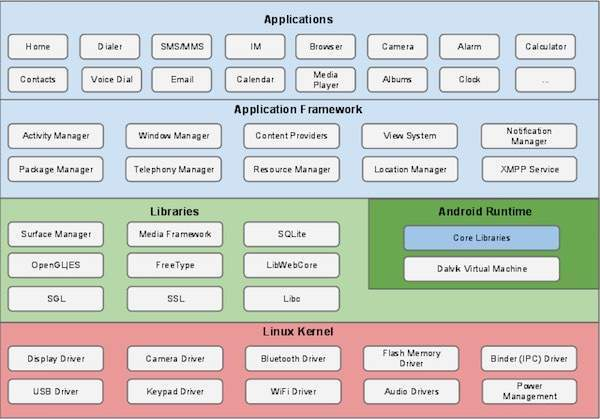
\includegraphics[width=\textwidth]{images/architecture.jpg}
    \caption{The Android OS structure} \label{fig1}
\end{figure}

\subsection{RiskInDroid Analysis Tool}
Analysis of the permissions is usually calculated empirically. An application is judged on a \textit{risk index value} out of 100.
The probabilistic risk index analysis approach for android applications is usually a good way to analyze the safety of an application.
RiskInDroid does quantitative risk analysis of android applications that are written in Java. It utilizes machine learning tools such as \textit{scikit-learn}
to generate a numeric risk index value between 0 and 100 for an application. Classifiers such as : \begin{itemize}
    \item Support Vector Machines (SVM)
    \item Multinomial Naive Bayes (MNB)
    \item Gradient Boosting (GB)
    \item Logistic Regression (LR)
\end{itemize}
are employed for classification. 

\textbf{RiskInDroid} takes into consideration both the permissions declares into the application manifest and the bytecode retrieved from the application through reverse engineering. Static analysis is used to classify the permissions used in the application into four different ways :
\begin{itemize}
    \item Declared permissions: which are extracted from the application manifest.
    \item Exploited permissions: declared and used in the bytecode.
    \item Ghost permissions: not declared but with usages in the bytecode.
    \item Useless permissions: they are declared but not used in the bytecode.
\end{itemize}

The risk value generated is considered to be accurate as it is trained upon 6000 malware samples and 112000 applications of varying levels of security.

\subsubsection{Analysis}
To execute the analysis, we are using : 
\begin{itemize}
    \item Ubuntu 20.04 LTS
    \item Docker 
    \item RiskInDroid Application
    \item Xiaomi Home Application for Analyis
\end{itemize}

\textbf{Instructions} :
\begin{itemize}
    \item git clone \url{https://github.com/ClaudiuGeorgiu/RiskInDroid.git}
    \item docker build -t riskindroid .
    \item docker run --rm -p 8080:80 riskindroid
\end{itemize}

The resulting RiskInDroid application is now running at localhost:8080. \ref{fig2}

\begin{figure}
    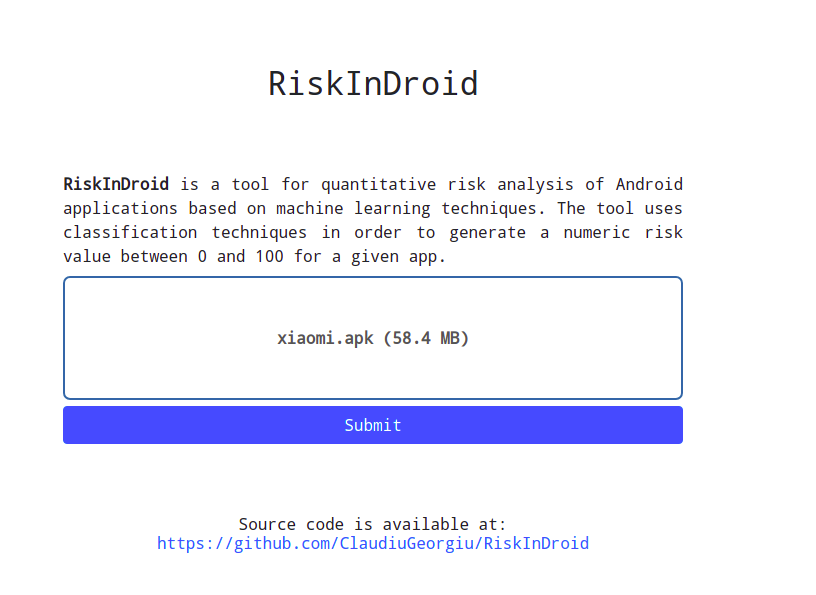
\includegraphics[width=\textwidth]{images/xiaomi-1.png}
    \caption{RiskInDroid Application} \label{fig2}
\end{figure}

\subsubsection{Results}
The Xiaomi application had a score of 30.34. \ref{fig3}.
The results related to permissions were :
\begin{itemize}
    \item Declared - 58 permissions.
    \item Required and Used - 21 permissions.
    \item Required but Not Used - 37 permissions.
    \item Not required but Used - 4 permissions.
\end{itemize}

Developers can use this to analyze the permissions to optimize the use, and thus improving the risk index.

\begin{figure}
    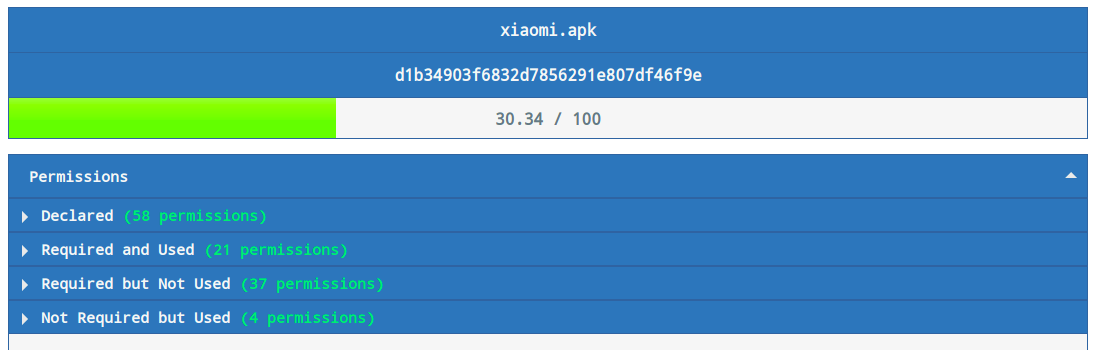
\includegraphics[width=\textwidth]{images/xiaomi-riskinDroid.png}
    \caption{RiskInDroid Application - Xiaomi Analysis} \label{fig3}
\end{figure}


\subsection{SPECK Tool}
As we saw in the previous section, analysis of an application can be done with permissions being provided to the android application. One more way to analyze the application is by using the code written to develop the application.
SPECK is a tool designed to search for bad/malicious coding practices in the android application. The software declares a specific set of rules to ensure the application's security. 

The many rules divide the intensity of the flaw into three levels : 
\begin{itemize}
    \item \textbf{INFO} : if a good coding practice is detected.
    \item \textbf{WARNING} : if there is an security issue which can be dangerous.
    \item \textbf{CRITICAL} : informs that there is a confirmed security issue.
\end{itemize}

To analyze an android application, we use the tool in developer mode. There are 32 different rules which will be used to analyze the coding practices of the android application.
The tools are based upon, 1) Best Practices 2) Security Tips 3) SSL Security 4) Configuration Security 5) Cryptography and 6) Direct Boot

The SPECK tool is downloaded and compiled. To analyze the Xiaomi application, we write \textit{python3 Scan.py -s path-to-xiaomi-app}
Manifest and the main java file in analyzed. The application analyzed \textbf{1719} files for the first rule.
In the \ref{fig4}, you see the analysis with Rule 8,9,10 which are : 
\begin{itemize}
    \item Rule 8 : Store private data within internal storage
    \item Rule 9 : Share data securely across apps
    \item Rule 10 : Use scoped directory access
\end{itemize}

A developer can read the output according to the different rules to improve the security of the application. 

\begin{figure}
    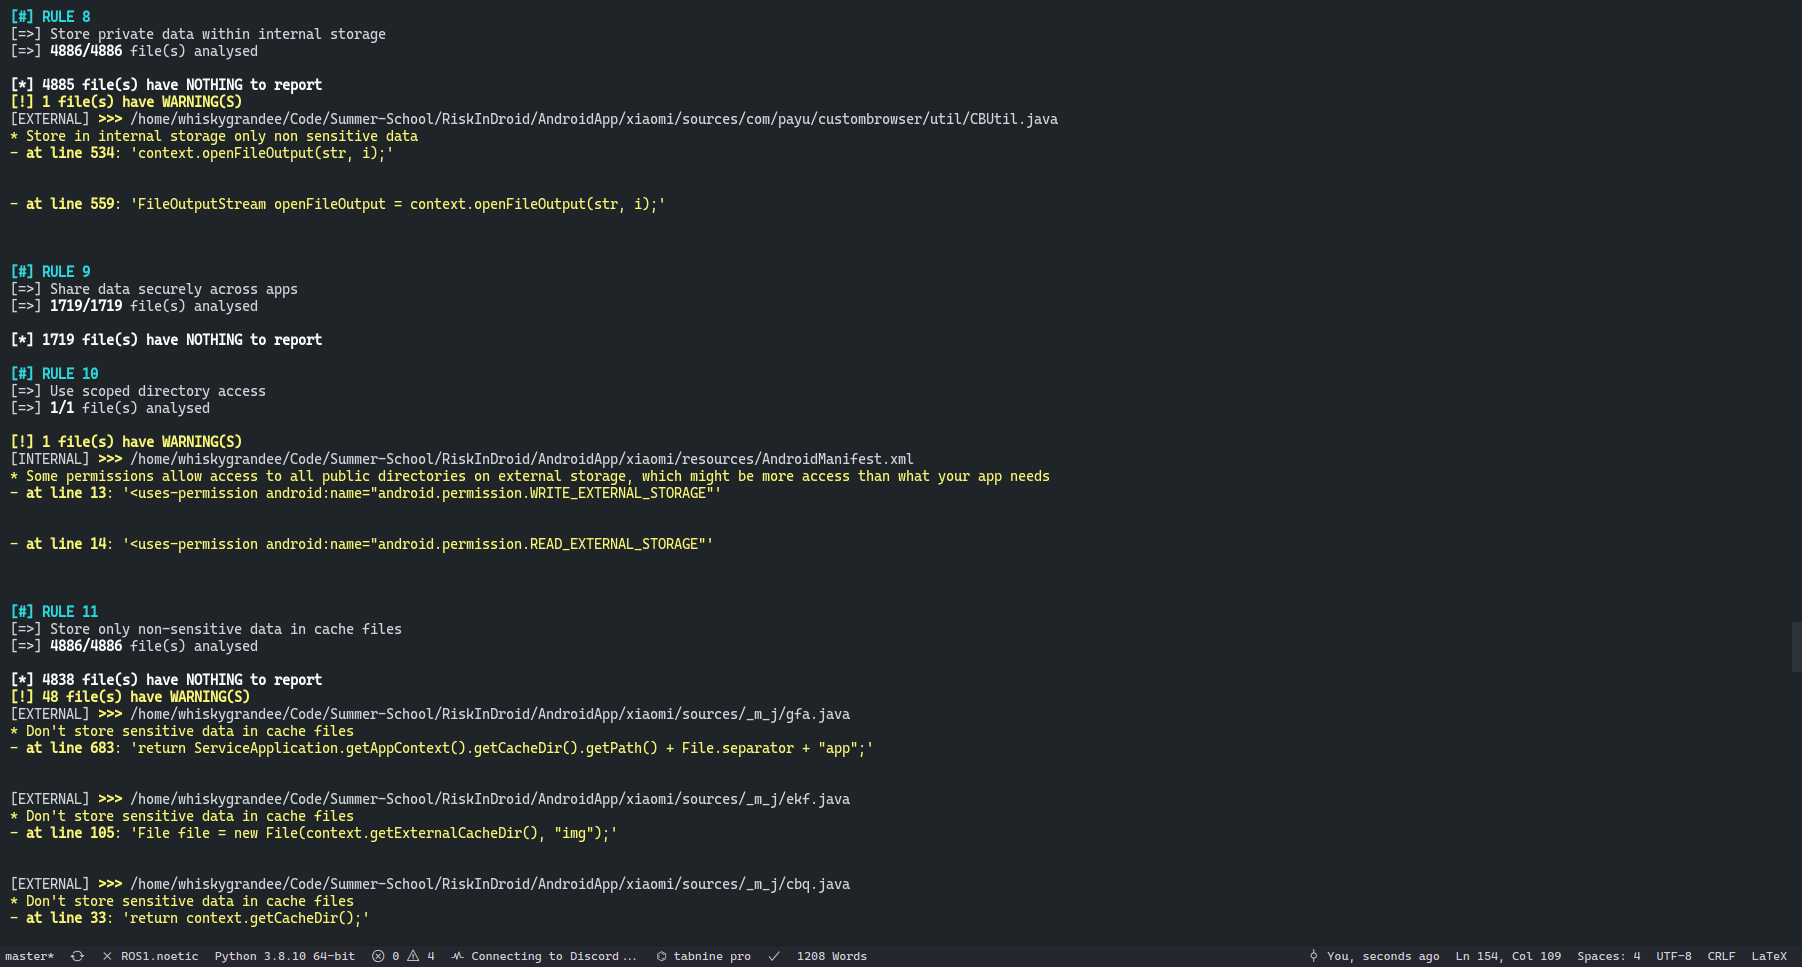
\includegraphics[width=\textwidth]{images/SPECK.png}
    \caption{SPECK Result - Xiaomi Analysis} \label{fig4}
\end{figure}

\section{Buffer Overflow in Cybersecurity}
Buffer Overflow is a \textit{trick} employed to induce a security flaw in a different system when we have a connection to it.
In the challenge, we studied Buffer Overflow and tried to connect to a different machine. We learn about memory, stack and then go through the process of 
Buffer Overflow. Tools used in the challenge were : 
\begin{itemize}
    \item A Virtual Machine running Windows 10
    \item VulnServer - a tool for making a server for vulnerability testing.
    \item Linux Machine - 20.04 Ubuntu LTS
    \item Immunity I/O Debugger tool.
\end{itemize}

By overflowing the buffer, we add extra data than memory can hold. This results in a discrepancy in the pattern of the bits. A buffer is a sequential section of memory allocated to contain a character string or integers. By overflowing it, the memory is corrupted and we can execute malicious code. It is a well-known form of software security vulnerability.
Such Cybersecurity vulnerabilities occur in code which : 
\begin{itemize}
    \item uses external data to do some action.
    \item employing poor coding qualities resulting in different scope of local and global variables.
    \item complexity that a programmer can not predict the behaviour.
\end{itemize}

Buffer Overflow was accomplished by following these steps : 

\begin{itemize}
    \item Spiking
    \item Fuzzing
    \item Finding the offset
    \item Overwriting the EIP
    \item Finding bad characters
    \item Finding the right module
    \item Generation of shellcode
    \item Access to Root.
\end{itemize}

\subsubsection{Spiking}
Attaching the VulnServer and starting it. We write a script to add a new string to the buffer. A spike script will send a lot of commands, i.e adding more and more strings to the buffer. We then find the particular command we need i.e \textbf{TRUN}. 

\subsubsection{Fuzzing}
As we now know the \textbf{TRUN} command to be utilized, we will send values only to that specific command. A python script will increase the buffer size to send to the command.
As long as we are connected to the other machine, we send the buffer. Whenever the program will crash due to overflow, a new byte will be added.
Information related to the end of the buffer i.e the byte will be printed out.

\subsubsection{Offset}
As we now know where the overflow has happened and the program has crashed, we will make another python script and use the pattern offset command to find an exact match of the offset.
The offset will decide where we will overwrite the EIP.

\subsubsection{Finding Bad Characters}
There will be a lot of bad characters or irregular characters in the buffer. We decide this by finding the irregularities in the continuous pattern in data.
We then use a bunch of EIF values to find anomalies in the HEX dump in the buffer.

\subsubsection{Finding the right module}
It exploits the program with no memory protection. There are various protection settings in the stack. 
We now locate the \textit{nasmshell()} to convert the assembly language to hex code. We controlled the EIP and the script produces a result
when it hits the EIP. A breakpoint is thus found.

\subsubsection{Generation of Shellcode and Access}
We employ msfvenom ( a tool to generate shellcode) and since we are targeting a windows machine we will let it be known in the command. 
Declaring a new variable to declare every hex code value in it. Shellcode is generated by using the offset and EIP and the overflow with padding.
We try figuring out the exploit till something works. As the connection is done, we generate the shellcode by running the script and we enter the Windows 10 shell by 
using buffer overflow.

\section{Cybersecurity UNIX Commands}
During the third day of summer school, Vilnius University Lithuania had a cyber security challenge related to UNIX command quizzes.
There were 7 quizzes for assessment during the summer school where I performed as :

\begin{table}
    \caption{Results from the Quizzes.}\label{tab2}
    \centering
    \begin{tabular}{|l|l|}
    \hline
    Quiz Number &  Grade \\
    \hline
    1.01 & 6/10 \\
    1.02 & 0.16/0.20 \\
    1.03 & 0.18/0.20 \\
    1.04 & 0.18/0.20 \\
    1.05 & 0.16/0.20 \\
    1.06 & 0.18/0.20 \\
    1.07 & 0.16/0.20 \\
    \hline
    \end{tabular}
\end{table}
During the challenges, questions were related to topics such as :
\begin{itemize}
    \item File Management
    \item Networking 
    \item Terminal Based Editors
    \item I/O Management
\end{itemize}

As the questions were multiple choice on the website, I will describe the major concepts which I learnt from them.
\subsubsection{File Management}
The file Management section dealt with various commands such as \textit{cd, pwd and ls} to get the information about the present file or folder. Further sections also asked questions related to \textit{time/history/copying files}. This section described the commands which will be used daily on operating a UNIX based system.
\subsubsection{Networking}
This section dealt with employing UNIX commands which will be used for networking based applications. IP configuration, pinging a website and connecting to a server with SHA was discussed and questions were asked related to this. Information related to this is very crucial in cyber security as you would use networking every time as that is the way you connect to either a different server or using commands in the network.
\subsubsection{Terminal Based Editors}
This section deals with teaching terminal-based editors such as QED and Vim and commands to copy/insert/delete characters and files and doing everything you would do to write code or commands to execute processes. As in cybersecurity, you will have to work with servers that work in UNIX.
Information about a terminal-based editor is crucial.
\subsubsection{I/O Management}
This section dealt with commands related to I/O management and interacting with different devices in the network.


\subsubsection{NOTE : } As all the questions in this challenge were online on Vilnius University's website and we don't have access to it after 
the summer school ended, I could not demonstrate all of the commands provided in the MCQs there. 

\section{Side Channel Analysis with Deep Learning}
Side Channel Analysis deals with Side-Channel Attacks in cybersecurity. It is based upon the information gained from the implementation of the information gained from the computer system.
It does not work with exploiting the weakness in the system or an algorithm implemented. They use electromagnetic leaks or power consumption and sound for that extra information to be exploited.

\begin{figure}
    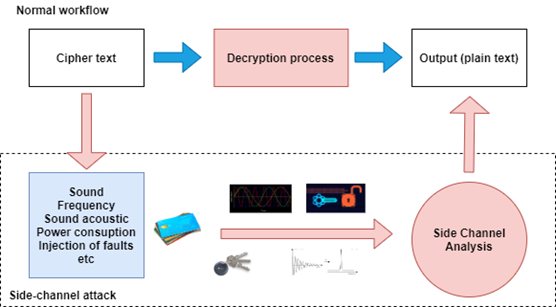
\includegraphics[width=\textwidth]{images/SCA.png}
    \caption{Side Channel Analysis} \label{fig8}
\end{figure}
\begin{figure}
    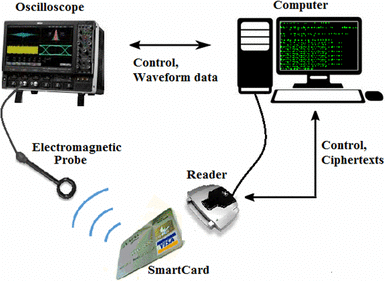
\includegraphics[width=0.8\textwidth]{images/Side-channel-analysis-materials.png}
    \caption{Side Channel Exploitation} \label{fig5}
\end{figure}
Side-Channel Attacks are employed in modern-day cyber security coupled up with the power of deep learning because the RSA based modern-day cryptography cyphers are too tough to crack.
The system is completely known except for the RSA key. The algorithm can be reverse-engineered or leaked by using the side-channel analysis. Side-channel analysis works with minimizing the secret 
information. 

NVIDIA-SMI 470.63.01    Driver Version: 460.32.03    CUDA Version: 11.2   was used as a graphic card for the challenge on Google Colab.
There are various sections in the challenge which we will talk about in the next sections.

\subsubsection{Simple Power Analysis}
Simple Power Analysis (SPA) is known as the simplest side-channel attack. It consists in exploiting the security flaws of a cryptographic module by observing one or very few leakage traces.
We are given a leakage trace coupled up with the time sample and we had to guess the private key. Using the traces, we find the private key.

\begin{figure}
    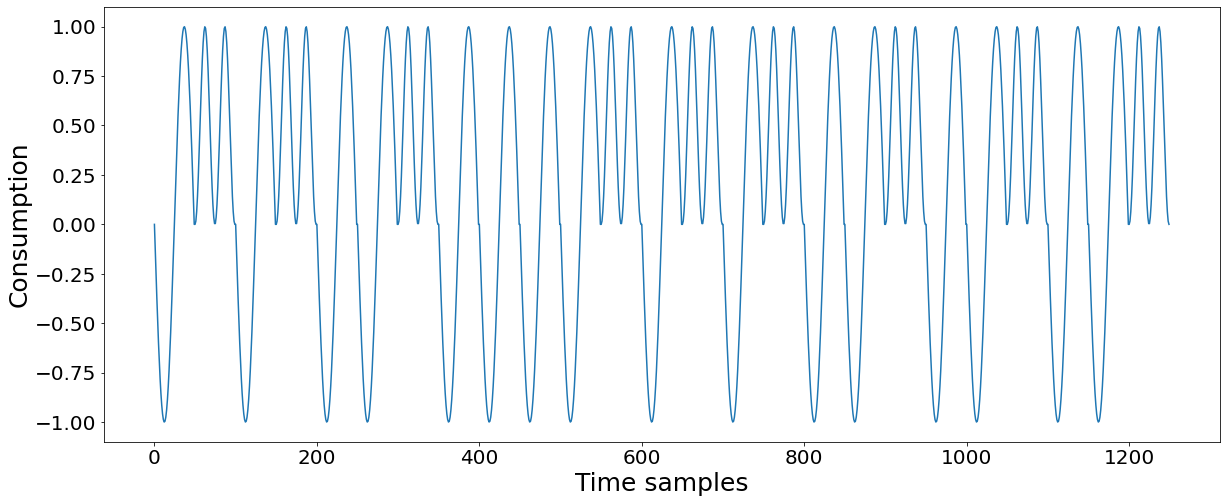
\includegraphics[width=\textwidth]{images/SPA.png}
    \caption{Simple Power Analysis - Traces} \label{fig6}
\end{figure}

\subsubsection{Differential Power Analysis}
When we target symmetric cryptographic algorithms, it results in multiple large numbers of power traces. Differential power analysis deals with
combining multiple power traces and leakage sources into one and then doing analysis on them. Differential power analysis gathers the information of multiple leakage traces constructed from different inputs. 
To assess the security of a cryptographic module, the Adversary can approximate the time sample where the sensitive information leaks (ie. Points of Interest (PoIs)). From an attack perspective, the leakage assessment is helpful to find the points of interest and evaluate the security flaws induced in a cryptographic module. Typically, the side-channel community considers the Signal-to-Noise Ratio (SNR) to detect those sensitive PoIs.
\begin{figure}
    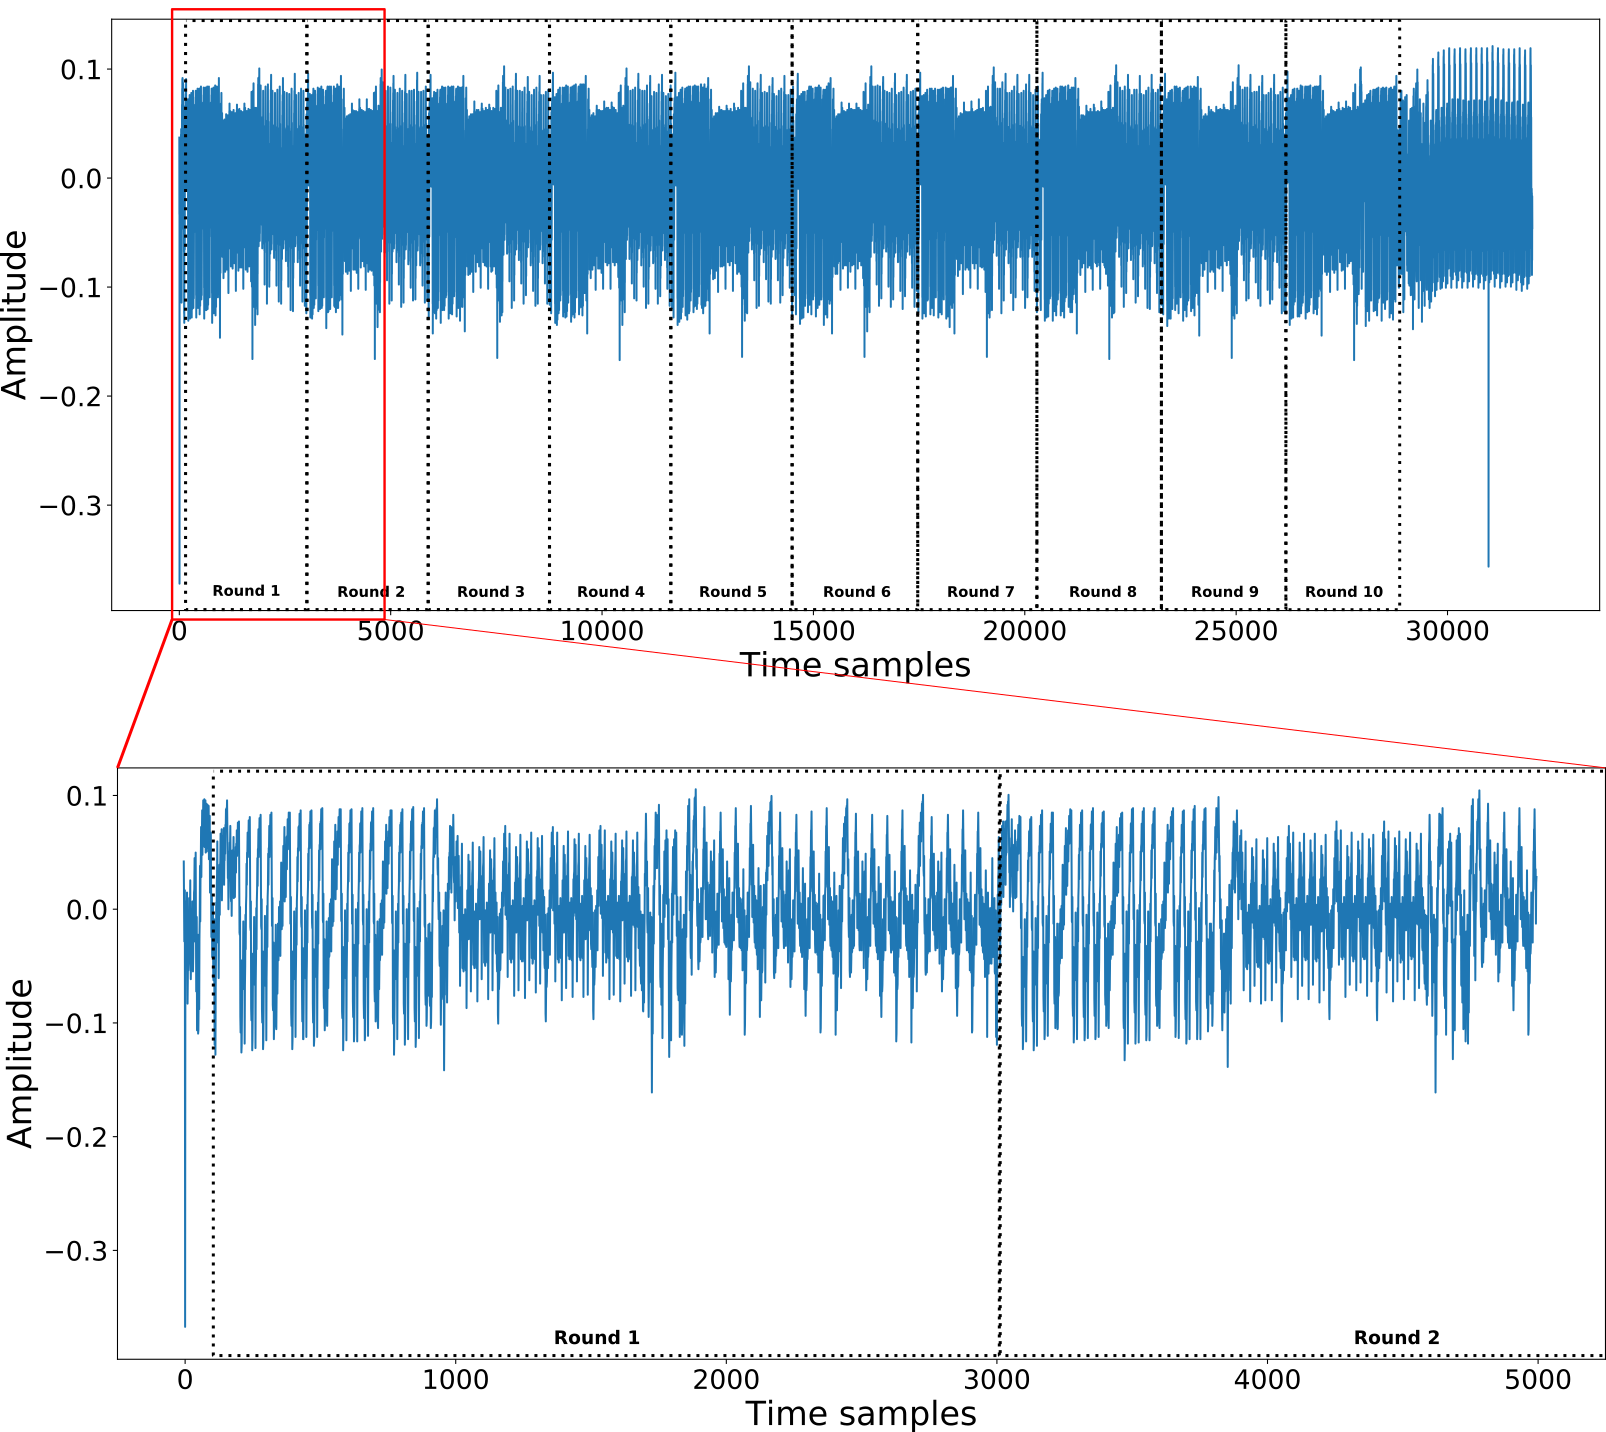
\includegraphics[width=\textwidth]{images/DPA.png}
    \caption{Differential Power Analysis - Traces} \label{fig7}
\end{figure}

\subsubsection{Side Channel Analysis on Desynchronized Data}
The hiding mechanisms are widely used as countermeasures that can be included in hardware or software cryptographic implementations. As defined in the course, the Adversary aims at identifying the time samples where the sensitive variable leaks to extract the information related to the manipulated secret key. The goal of hiding is to distribute the execution of the sensitive variables over a different period. The distribution should neither be predictable nor be observable by the Adversary. If the leakage traces are perfectly synchronized, the probability of observing the execution of a given cryptographic operation for some time is nearly  1  while the hiding mechanisms reduce this probability. The higher the hiding level, the lesser the probability of observing the execution of a given cryptographic operation for a certain period. Therefore, it significantly reduces the correlation between the targeted sensitive variable and the time samples where it leaks. This countermeasure reduces the Signal-to-Noise Ratio by increasing the related noise without eliminating the informative signal itself.

\section{Conclusion}
During a week I understood that cybersecurity is an interesting field. I learnt that cybersecurity is much more than just hacking web pages, including deep learning and using power analysis to crack encryption is an amazing insight I received during the week. 
I wish to further learn the skills taught during school whenever I find time in leisure. I thank ARQUS for conducting the summer school as well as participating universities and professors involved who took their time to share the knowledge.
\end{document}
